\documentclass{article}
\usepackage[utf8]{inputenc}
\usepackage[T2A]{fontenc}
\usepackage[russian]{babel}
\usepackage{amsthm}
\usepackage{amssymb}
% \usepackage{tikz}
\usepackage{textcomp}
% \usepackage{marvosym}
% \usepackage{ esint }
\usepackage{graphicx}\usepackage{amsfonts}
\setlength{\topmargin}{-0.5in}
\setlength{\textheight}{9.1in}
\setlength{\oddsidemargin}{-0.4in}
\setlength{\evensidemargin}{-0.4in}
\setlength{\textwidth}{7in}
\setlength{\parindent}{0ex}
\setlength{\parskip}{1ex}
\begin{document}

\renewcommand{\abstractname}{Полный анализ функции}\begin{abstract}Данный документ содержит полный анализ функции с разложением в ряд Тейлора и построением графика\end{abstract}
\section{Взятие 2-ой производной.}

$ f(x) = {(\sin(x))}^{5} + \cos(x)$

Заметим, что:

${({(\sin(x))}^{5} + \cos(x))}^{'} = {({(\sin(x))}^{5})}^{'} + {(\cos(x))}^{'}$

Не требует дальнейших комментариев:

${(\cos(x))}^{'} = - \sin (x) \cdot{(x)}^{'}$

Нетрудно заметить:

${(x)}^{'} = 1$

Очевидно, что:

${({(\sin(x))}^{5})}^{'} = 5\cdot {\sin(x)}^{5 - 1} \cdot{(\sin(x))}^{'}$

Заметим, что:

${(\sin(x))}^{'} = cos(x) \cdot{(x)}^{'}$

Очевидно, что:

${(x)}^{'} = 1$

Нетрудно заметить:

${(5 \cdot {(\sin(x))}^{4} \cdot \cos(x) + (-1) \cdot \sin(x))}^{'} = {(5 \cdot {(\sin(x))}^{4} \cdot \cos(x))}^{'} + {((-1) \cdot \sin(x))}^{'}$

Нетрудно заметить:

${((-1) \cdot \sin(x))}^{'} = {((-1))}^{'}\cdot \sin(x) + (-1)\cdot {(\sin(x))}^{'}$

Нетрудно заметить:

${(\sin(x))}^{'} = cos(x) \cdot{(x)}^{'}$

Очевидно, что:

${(x)}^{'} = 1$

Заметим, что:

${((-1))}^{'} = 0$

Заметим, что:

${(5 \cdot {(\sin(x))}^{4} \cdot \cos(x))}^{'} = {(5 \cdot {(\sin(x))}^{4})}^{'}\cdot \cos(x) + 5 \cdot {(\sin(x))}^{4}\cdot {(\cos(x))}^{'}$

Заметим, что:

${(\cos(x))}^{'} = - \sin (x) \cdot{(x)}^{'}$

Не требует дальнейших комментариев:

${(x)}^{'} = 1$

Заметим, что:

${(5 \cdot {(\sin(x))}^{4})}^{'} = {(5)}^{'}\cdot {(\sin(x))}^{4} + 5\cdot {({(\sin(x))}^{4})}^{'}$

Не требует дальнейших комментариев:

${({(\sin(x))}^{4})}^{'} = 4\cdot {\sin(x)}^{4 - 1} \cdot{(\sin(x))}^{'}$

Не требует дальнейших комментариев:

${(\sin(x))}^{'} = cos(x) \cdot{(x)}^{'}$

Нетрудно заметить:

${(x)}^{'} = 1$

Не требует дальнейших комментариев:

${(5)}^{'} = 0$

Получаем:

$ f^{(2)}(x) = (0 \cdot {(\sin(x))}^{4} + 5 \cdot 4 \cdot {(\sin(x))}^{(4 - 1)} \cdot \cos(x) \cdot 1) \cdot \cos(x) + 5 \cdot {(\sin(x))}^{4} \cdot \sin(x) \cdot (-1) \cdot 1 + 0 \cdot \sin(x) + (-1) \cdot \cos(x) \cdot 1$

\section{Упрощение.}

$(0 \cdot {(\sin(x))}^{4} + 5 \cdot 4 \cdot {(\sin(x))}^{(4 - 1)} \cdot \cos(x) \cdot 1) \cdot \cos(x) + 5 \cdot {(\sin(x))}^{4} \cdot \sin(x) \cdot (-1) \cdot 1 + 0 \cdot \sin(x) + (-1) \cdot \cos(x) \cdot 1 = 5 \cdot 4 \cdot {(\sin(x))}^{3} \cdot \cos(x) \cdot \cos(x) + 5 \cdot {(\sin(x))}^{4} \cdot (-1) \cdot \sin(x) + (-1) \cdot \cos(x)$
\section{Вычисление значения функции в точке.}

$ f(10) = -0.886723 $
\section{Вычисление производной функции в точке.}

$ f^{'}(5) = 2.3514 $
\section{Разложение данной функции в ряд Тейлора.}

${(\sin(x))}^{5} + \cos(x) =  1 - \frac{1}{2}\cdot x^2 + \frac{1}{24}\cdot x^4 + \frac{120}{120}\cdot x^5 - \frac{1}{720}\cdot x^6 - \frac{4200}{5040}\cdot x^7 + o(x^7) $
\section{Уравнение касательной функции в точке x = 2.}

g(x) = $-2.33176 \cdot x + 4.869 $
\section{График функции и касательной к ней.}


\begin{figure}[ht]
\center
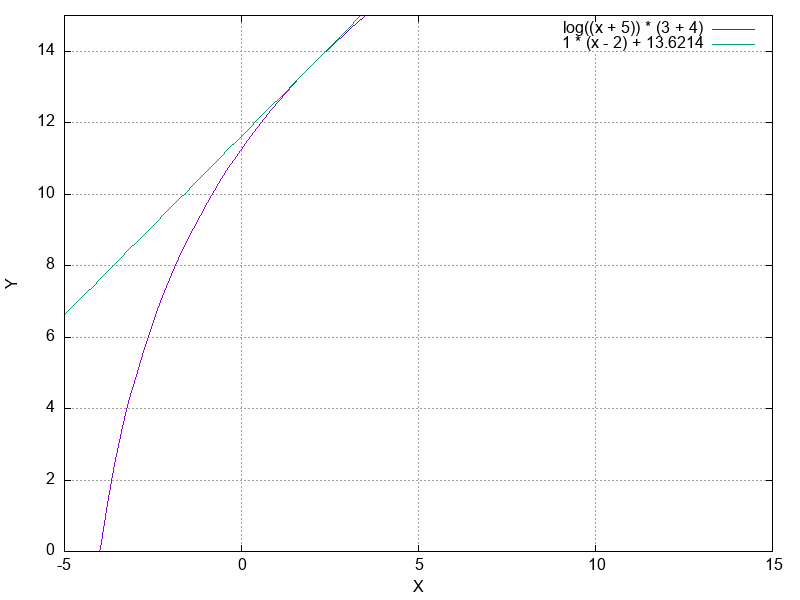
\includegraphics[scale=0.65]{graph.png}
\end{figure}
\end{document}